% An ear decomposition (generated by figs_c1ch05.py).
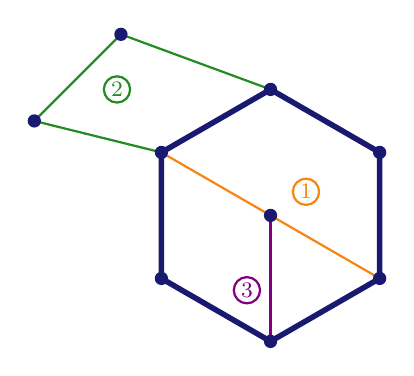
\begin{tikzpicture}[x=1cm,y=1cm,v/.style={circle,fill=MidnightBlue,inner sep=1.8pt},c/.style={line width=2pt,MidnightBlue},n/.style={circle,draw,thick,inner sep=1pt,font=\footnotesize,fill=white}]
\coordinate (a0) at (0.000,1.600);
\coordinate (a1) at (-1.386,0.800);
\coordinate (a2) at (-1.386,-0.800);
\coordinate (a3) at (-0.000,-1.600);
\coordinate (a4) at (1.386,-0.800);
\coordinate (a5) at (1.386,0.800);
\coordinate (x) at (0.000,0.000);
\coordinate (y) at (-1.900,2.300);
\coordinate (z) at (-3.000,1.200);
\draw[c] (a0) -- (a1) -- (a2) -- (a3) -- (a4) -- (a5) -- cycle;
\draw[thick,BurntOrange] (a1) -- (x) -- (a4); \node[n,draw=BurntOrange,text=BurntOrange] at (0.45,0.3) {1};
\draw[thick,ForestGreen] (a0) -- (y) -- (z) -- (a1); \node[n,draw=ForestGreen,text=ForestGreen] at (-1.95,1.6) {2};
\draw[thick,Purple] (x) -- (a3); \node[n,draw=Purple,text=Purple] at (-0.3,-0.95) {3};
\fill[MidnightBlue] (a0) circle (2.4pt);
\fill[MidnightBlue] (a1) circle (2.4pt);
\fill[MidnightBlue] (a2) circle (2.4pt);
\fill[MidnightBlue] (a3) circle (2.4pt);
\fill[MidnightBlue] (a4) circle (2.4pt);
\fill[MidnightBlue] (a5) circle (2.4pt);
\fill[MidnightBlue] (x) circle (2.4pt);
\fill[MidnightBlue] (y) circle (2.4pt);
\fill[MidnightBlue] (z) circle (2.4pt);
\end{tikzpicture}
